\documentclass[final]{fhnwreport}       %[mode] = draft or final
                                        %{class} = fhnwreport, article, 
                                        %          report, book, beamer, standalone
%%---Main Packages-----------------------------------------------------------------------
\usepackage[english, ngerman]{babel}	%Mul­tilin­gual sup­port for LaTeX
\usepackage[T1]{fontenc}				%Stan­dard pack­age for se­lect­ing font en­cod­ings
\usepackage[utf8]{inputenc}				%Ac­cept dif­fer­ent in­put en­cod­ings
\usepackage{lmodern}                    %The newer Font-Set
\usepackage{textcomp}					%LaTeX sup­port for the Text Com­pan­ion fonts
\usepackage{graphicx} 					%En­hanced sup­port for graph­ics
\usepackage{float}						%Im­proved in­ter­face for float­ing ob­jects
\usepackage{ifdraft}                    %Let you check if the doc is in draft mode

%%---Useful Packages---------------------------------------------------------------------
\usepackage[pdftex,dvipsnames,table]{xcolor}  %Driver-in­de­pen­dent color ex­ten­sions for LaTeX
\usepackage{csquotes}                   %Simpler quoting with \enquote{}
\usepackage{siunitx} 					%A com­pre­hen­sive (SI) units pack­age
\usepackage{listings}					%Type­set source code list­ings us­ing LaTeX
\usepackage[bottom]{footmisc}			%A range of foot­note op­tions
\usepackage{footnote}					%Im­prove on LaTeX's foot­note han­dling
\usepackage{verbatim}					%Reim­ple­men­ta­tion of and ex­ten­sions to LaTeX ver­ba­tim
\usepackage[textsize=footnotesize]{todonotes} %Mark­ing things to do in a LaTeX doc­u­ment
\usepackage{booktabs}
\usepackage{lscape}
\usepackage{blindtext}
\usepackage{wrapfig}

%%---Tikz Packages-----------------------------------------------------------------------
\usepackage{standalone}
\usepackage{tikz}
\usepackage{circuitikz}
\usetikzlibrary{arrows}
\usetikzlibrary{calc}
\usetikzlibrary{intersections}

%%---Math Packages-----------------------------------------------------------------------
\usepackage{amsmath}					%AMS math­e­mat­i­cal fa­cil­i­ties for LaTeX
%\usepackage{amssymb}					%Type­set­ting symbols (AMS style)
%\usepackage{array}						%Ex­tend­ing the ar­ray and tab­u­lar en­vi­ron­ments
%\usepackage{amsthm}					%Type­set­ting the­o­rems (AMS style)

%%---Table Packages----------------------------------------------------------------------
\usepackage{tabularx}					%Tab­u­lars with ad­justable-width columns
%\usepackage{longtable}
\usepackage{multirow}					%Create tab­u­lar cells span­ning mul­ti­ple rows
\usepackage{multicol}					%In­ter­mix sin­gle and mul­ti­ple columns

%%---PDF / Figure Packages---------------------------------------------------------------
\usepackage{pdfpages}					%In­clude PDF doc­u­ments in LaTeX
\usepackage{pdflscape}					%Make land­scape pages dis­play as land­scape
\usepackage{subfig}					    %Fig­ures di­vided into sub­fig­ures

%%---Other Packages----------------------------------------------------------------------
%\usepackage{xargs}                     %De­fine com­mands with many op­tional ar­gu­ments

%%---Bibliography------------------------------------------------------------------------
\bibliographystyle{unsrt}

%%---Main Settings-----------------------------------------------------------------------
\graphicspath{{./graphics/}}			%Defines the graphicspath
%\geometry{twoside=false}				    %twoside=false disables the "bookstyle"
\setlength{\marginparwidth}{2cm}
\overfullrule=5em						%Creates a black rule if text goes over the margins => debugging


%%---User Definitions--------------------------------------------------------------------
%%Tabel-Definitions: (requires \usepackage{tabularx})
\newcolumntype{L}[1]{>{\raggedright\arraybackslash}p{#1}}    %column-width and alignment
\newcolumntype{C}[1]{>{\centering\arraybackslash}p{#1}}
\newcolumntype{R}[1]{>{\raggedleft\arraybackslash}p{#1}}

%%---Optional Package Settings-----------------------------------------------------------
%Listings-Settings: (requires \usepackage{listings}) => Example with Matlab Code
\lstset{language=Matlab,%
    basicstyle=\footnotesize\ttfamily,
    breaklines=false,%
    morekeywords={switch, case, otherwise},
    keywordstyle=\color{Blue},%
    tabsize=2,
    %morekeywords=[2]{1}, keywordstyle=[2]{\color{black}},
    identifierstyle=\color{Black},%
    stringstyle=\color{Purple},
    commentstyle=\color{Green},%
    showstringspaces=false,%without this there will be a symbol in the places where there is a space
    numbers=left,%
    numberstyle={\tiny \color{black}},% size of the numbers
    numbersep=9pt, % this defines how far the numbers are from the text
    %emph=[1]{word1, word2,...},emphstyle=[1]\color{red}
}										                %loads all packages, definitions and settings												
\title{\Huge{\textbf{Fachbericht}}\\}          %Project Title
\author{\huge{Wetterstation mit Solar Energie}}          %Document Type => Technical Report, ...
\date{Windisch, \today}             %Place and Date


\begin{document}

%%---TITLEPAGE---------------------------------------------------------------------------
\selectlanguage{ngerman}                %ngerman or english
\maketitle
%\vspace*{-1cm}
\vspace*{-0.5cm}						    %compensates the space after the date line.
\vfill
\begin{figure}[H]
\centering
%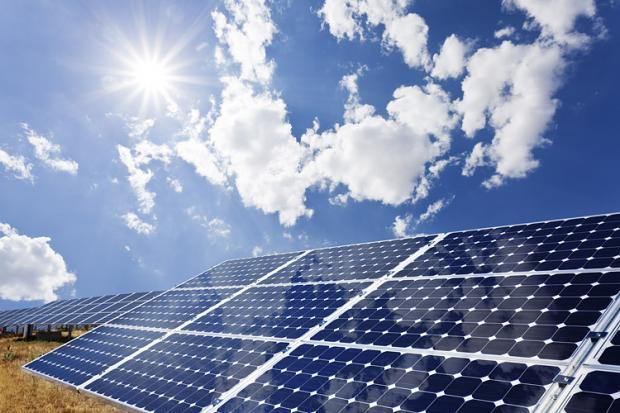
\includegraphics[width=\linewidth]{Titelbild.jpg}
\end{figure}
\vfill

{
\renewcommand\arraystretch{2}
\begin{center}
\begin{tabular}{>{\bf}p{4cm} l}
Hochschule                 &    Hochschule für Technik - FHNW\\
Studiengang                &    Elektro- und Informationstechnik\\
Autor/-en  		           & 	Mischa Knupfer, Andres Minder\\
Betreuer                   &    Prof. Dr. Taoufik Nouri\\
Auftraggeber               &    Prof. Dr. Taoufik Nouri\\
Version                    &    1.0 %Normally not used!
\end{tabular}
\end{center}
}

\clearpage
			
%%---ABSTRACT----------------------------------------------------------------------------
\selectlanguage{english}				%ngerman or english
\thispagestyle{empty}
\begin{abstract}

\end{abstract}	

%%---TABLE OF CONTENTS-------------------------------------------------------------------
\pagenumbering{Roman}		
\selectlanguage{ngerman}				%ngerman or english
\tableofcontents
\clearpage

%%---TEXT--------------------------------------------------------------------------------
\pagenumbering{arabic}
Einleitung
\section{Auftragsbeschreibung}
Das Wetter spielt eine wichtige Rolle in der Agronomie. Regnet es nicht genug, müssen Pflanzen bewässert werden. Trifft auf ein Ort nur wenig Sonnenlicht, so sollten dort nicht die Pflanzen, welche viel Sonnenlicht brauchen, angebaut werden. Windet es zu stark, können Pflanzen beschädigt oder gar zerstört werden. Ist es Tagsüber heiss, so benötigen die Pflanzen mehr Wasser. Hiesige Bauern besitzen den Luxus von guten Wettervorhersagen dank dem Bundesamt für Meteorologie und Klimatologie (MeteoSchweiz). Dieser Luxus ist in anderen Ländern noch nicht gegeben. Prof. Dr. Nouri Taoufik ist aufgefallen, dass in tropischen Gegenden wie Südamerika oder teile Afrikas dieser Luxus ebenso fehlt. \\[0.5cm]
Aus diesem Grund soll eine kostengünstige, erweiterbare und mobile Wetterstation entwickelt werden, welche diese Bauern unterstützt. Diese Wetterstation soll die Regenmenge, die Windstärke, die Lufttemperatur und die Sonnenstunden messen können. Ausserdem soll die Wetterstation mittels Photovoltaik unterstützt werden, und erhobene Daten via SMS abrufbar sein. \\[0.5cm]

\begin{landscape}
\section{Ziele}
Die Ziele sind strikt aufgeteilt in die zwei Projekte 5 und 6. Darin enthalten sind die jeweiligen zu erreichenden Muss- und Wunschziele mit ihren quantifizierten Spezifikationen. Diese sind wichtig, da Ortsabhängig unterschiedliche Normwerte gelten und sich dieses Projekt grundsätzlich auf die Schweiz fokussiert.\\
\begin{table}[htbp]
  \centering
  %\small
  \caption{Ziele P5}
    \begin{tabular}{r|l|r|l|l}
          & \textbf{Ziel} & \multicolumn{1}{l|}{\textbf{Messbereiche}} & \textbf{Genauigkeiten} & \textbf{Einheiten} \\
    \toprule
    \multicolumn{1}{l}{\textbf{Mussziele P5}} & \multicolumn{1}{r}{} & \multicolumn{1}{r}{} & \multicolumn{1}{r}{} &  \\
    \toprule
    \multicolumn{1}{l|}{Sensoren} & Lufttemperaturmessung & \multicolumn{1}{l|}{[-20;60]} & $\pm$ 1 & $^\circ$C \\
\cline{2-5}          & Windgeschwindigkeitsmessung & \multicolumn{1}{l|}{[10;25]} & $\pm$ 1   & m/s \\
\cline{2-5} & Niederschlagsmenge &   Wasser    & $\pm$ 100 & ml/m$^2$ \\
    \hline
    \multicolumn{1}{l|}{Datenspeicherung} & Datenabfrage via PuTTY &   $\geq$ 9600    &       &  Bd/s\\
    \hline
    \multicolumn{1}{l|}{RTC} & Implementation &   Echtzeit    & $\pm$ 1   & s/Jahr \\
\bottomrule
\multicolumn{1}{l}{\textbf{Wunschziele P5}} & \multicolumn{1}{l}{} & \multicolumn{1}{l}{} & \multicolumn{1}{l}{} &  \\
    \toprule
    \multicolumn{1}{l|}{Sensoren} & Sonnenstunden Prototyp &   Echtzeit    &       & s \\
    \bottomrule
    \end{tabular}%
  \label{tab:ZieleP5}%
\end{table}%

Tabelle \ref{tab:ZieleP5} zeigt diverse Ziele im P5, unterteilt in Muss- und Wunschziele. Zu den Musszielen gehören die Lufttemperaturmessung, die Windgeschwindigkeitsmessung, die Niederschlagsmessung, die Implementation des RTC und die mögliche Datenabfrage via Putty vom Datenspeicher. Die Lufttemperatur soll zwischen -20 bis 60 $^\circ$C ermittelbar sein, mit einer Genauigkeit von $\pm$1 $^\circ$C. Die Windgeschwindigkeitsmessung soll vor allem stärkere Windgeschwindigkeiten erfassen, um vor Sturm warnen zu können, weshalb niedrigere Windgeschwindigkeiten vernachlässigt werden können. Die Windgeschwindigkeit soll zwischen 10 und 25 m/s auf $\pm$1 m/s genau gemessen werden. Die Niederschlagsmenge soll nur für Regenwasser bestimmt werden mit einer Genauigkeit von $\pm$100 ml/m$^2$. Als Wunschziel soll eine Möglichkeit getestet werden um Sonnenstunden zu detektieren, welche dann im P6 umgesetzt wird.\\

\newpage
% Table generated by Excel2LaTeX from sheet 'Tabelle1'
\begin{table}[htbp]
  \centering
  %\small
  \caption{Ziele P6}
    \begin{tabular}{l|l|r|r|r}
          & \textbf{Ziel} & \multicolumn{1}{l|}{\textbf{Messbereiche}} & \multicolumn{1}{l|}{\textbf{Genauigkeiten}} & \multicolumn{1}{l}{\textbf{Einheiten}} \\
    \toprule
    \multicolumn{1}{l}{\textbf{Mussziele P6}} & \multicolumn{1}{r}{} & \multicolumn{1}{r}{} & \multicolumn{1}{r}{} &  \\
    \toprule
    Speisung & Akkukapazität &       &       &  \\
\cline{2-5}          & Ladeschaltung Akku &       &       &  \\
\cline{2-5}           & Ladeschaltung Photovoltaik &       &       &  \\
    \hline
    Kommunikationsmodul & GPS   &       &       &  \\
\cline{2-5}          & Mobilfunk (SMS) &       &       &  \\
\hline
Sensoren & Sonnenstunden &       &       &  \\
    \bottomrule
    \multicolumn{1}{l}{\textbf{Wunschziele P6}} & \multicolumn{1}{r}{} & \multicolumn{1}{r}{} & \multicolumn{1}{r}{} &  \\
    \toprule
    Kommunikationsmodul & Mobilfunk (Website) &       &       &  \\
    \hline
    Speisung & Akku austauschbar &       &       &  \\
    \bottomrule
    \end{tabular}%
  \label{tab:ZieleP6}%
\end{table}%

\noindent
Tabelle \ref{tab:ZieleP6} zeigt diverse Ziele im P6, unterteilt in Muss- und Wunschziele. Diese Tabelle ist unvollständig und wird im P6 nachgeführt. Generell kann gesagt werden, dass die Speisung, das Kommunikationsmodul mit GPS und Mobilfunk, sowie die Sonnenstunden-Sensorik implementiert werden sollen. Als Wunschziele sind ein austauschbarer Akku und eine Website zur Datensicherung und ggf. grafischen Darstellung aufgeführt.
\end{landscape}

\section{MCU}
Die Micro Controller Unit (MCU) ist der zentrale Bestandteil für die Kommunikation, resp. für den Datenaustausch zwischen den unterschiedlichen Modulen. Sie interpretiert die Signale der Sensoren und rechnet sie in die interessierenden Messwerte um. Dann weist die MCU jedem Messwert einen Zeitstempel über das RTC zu und übergibt diesen der Datenspeicherung. Wenn die Daten vom Kommunikationsmodul angefordert werden, liest die MCU die Datenspeicherung aus und übergibt sie dem Kommunikationsmodul.\\

{\begin{minipage}[b][130pt][t]{0.5\textwidth}
Für die Entwicklung der MCU wird ein Arduino Mega Board verwendet. Der Vorteil besteht darin, dass elementare Bauteile (Hardware) bereits implementiert sind, wie z.B. Oszillator, der USB-Anschluss und die PCB-Connectors für ein schnelles Prototyping. Die wichtigsten technischen Daten sind in der Tabelle \ref{tab:arduinoMega_technischeDaten} aufgelistet.\\
\end{minipage}}
\hfill
{\begin{minipage}[b][130pt][t]{0.49\textwidth}
\centering
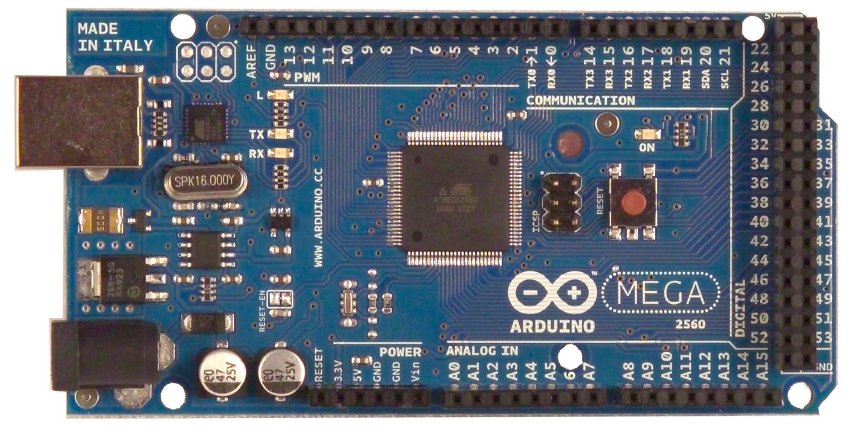
\includegraphics[width=0.99\textwidth]{graphics/MCU/arduino_mega.png}
\captionof{figure}{Arduino Mega Board \cite[S.1]{arduinoMega}}
\label{fig:arduinoMega}
\end{minipage}}

\begin{table}[h]
\centering
\caption{Technische Daten \cite[S.3]{arduinoMega}}
\begin{tabular}{|l|l|}
\hline 
Microcontroller & ATmega2560 \\ 
\hline 
Operating Voltage & 5V \\ 
\hline 
Digital I/O Pins & 54  \\ 
\hline 
Analog Input Pins & 16 \\ 
\hline 
Flash Memory & 256 KB, 8 KB werden vom bootloader benötigt\\ 
\hline 
SRAM & 8 KB \\ 
\hline 
EEPROM & 4 KB \\ 
\hline 
Clock Speed & 16 MHz \\ 
\hline 
\end{tabular}
\label{tab:arduinoMega_technischeDaten}
\end{table}

\section{RTC}

\section{Sensoren}


\subsection{Messen der Lufttemperatur}
\subsection{Ermittlung der Niederschlagsmenge}
Dieses Unterkapitel befasst sich mit der Realisierung der Niederschlagsmessung. Diese soll nach einem Kipplöffelprinzip funktionieren und gemäss definierten Zielen eine Genauigkeit von $\pm$100 ml/$m^2$ aufweisen. Ausserdem soll als alternative zusätzlich ein Messbecher an der Wetterstation installiert werden, damit der Bauer die Niederschlagsmenge anhand einer Skala ablesen kann. In einem ersten Schritt soll das Kipplöffelprinzip näher erläutert werden. Darauf folgend sollen die Realisierung dieses Kipplöffels und anschliessend die Implementation in der Firmware thematisiert werden. Zu guter Letzt soll die Validierung des Teilsystems folgen.
\subsubsection*{Das Kipplöffelprinzip}
Das Prinzip des Kipplöffels wird in Abbildung \ref{fig:Kipp} graphisch dargestellt.

\begin{figure}[h]
\centering
\includegraphics[width=0.8\linewidth]{graphics/Kipploeffel.png}
\caption{Darstellung des Kipplöffelprinzips}
\label{fig:Kipp}
\end{figure}

Abbildung \ref{fig:Kipp} zeigt das Kipplöffelprinzip. Der Kipplöffel (\glqq 3)\grqq) besteht im Grunde aus zwei Löffeln und ist in der Mitte drehbar mit dem Gehäuse befestigt (\glqq 4)\grqq). Regenwasser wird über eine Öffnung im Gehäusedeckel (Trichter, \glqq 1)\grqq) zum Kipplöffel befördert (\glqq 2)\grqq). Ist der Löffel mit Regenwasser gefüllt, so kippt dieser aufgrund des Gewichts und leert das Wasser über eine Öffnung im Gehäuseboden (\glqq 5)\grqq) aus. Durch die Kippung wird der andere Löffel in die Ausgangsposition bewegt und kann sich nun mit Wasser füllen. Mit der Hilfe von Reedkontakten und Magneten wird die Anzahl der Kippbewegungen gezählt. Die Niederschlagsmenge ergibt sich aus der Anzahl Kippbewegungen, multipliziert mit dem Volumen des Kipplöffels.
\subsubsection*{Die Realisierung des Niederschlagsmengensensors}
Der Niederschlagsmengensensor wird, wie im Pflichtenheft festgehalten, selbst erstellt. Die Erstellung kann in vier Etappen unterteilt werden. Die erste Etappe ist die Erstellung des Kipplöffels. Die zweite Etappe folgt mit der Erstellung der Drehbaren Lagerung. Als dritte Etappe folgt der Trichter und die vierte und letzte Etappe widmet sich dem Gehäuse.
\paragraph{Die Realisierung des Kipplöffels}
Wichtig für die Erstellung des Kipplöffels sind die Dimensionierung und die Materialwahl.
 
Das Material soll wetterbeständig, einfach bearbeitbar und günstig sein und eine möglichst glatte Oberfläche haben. Die möglichst glatte Oberfläche ist notwendig, damit das Wasser im Kipplöffel sich nicht an der Oberfläche festhält und somit gut abfliesst. Acrylglas erfüllt diese Bedingungen und ist in jedem Baumarkt erhältlich, weshalb es als Material gewählt wird.

Die Dimensionierung ist Abhängig von der gewählten Auflösung im Pflichtenheft. Damit eine Auflösung von $\pm$100 ml/$m^2$ erreicht werden kann, müssen beide Löffel des Kipplöffels bei genau 100 ml Fassungsvermögen kippen. Damit dies erreicht wird, kann man physikalisch die statische Gleichgewichtsbedingung aufstellen und daraus die Dimensionierung folgern. Dies ist jedoch ein sehr aufwändiger, komplizierter und zeitintensiver weg. Einfacher ist es, wenn der Kipplöffel extra zu gross dimensioniert und die Füllmenge im nachhinein justiert wird. Die Justierung erfolgt mittels einer in der Höhe verstellbaren Lagerung, sowie mit in der Höhe verstellbaren Schrauben im Gehäuseboden, welche die Neigung der Endposition des Kipplöffels beeinflusst. Ein weiterer Vorteil dieser Nachjustierung ist, dass auch eine andere Füllmenge einstellbar wäre.

\paragraph{Die Realisierung der drehbaren Lagerung des Kipplöffels}
Die Drehbare Lagerung des Kipplöffels ist wichtig, damit der Kipplöffel auf beide Seiten kippen kann. Die Drehachse soll direkt unterhalb der Mitte des Kipplöffels befestigt sein um ein gleichmässiges Kippen zu ermöglichen. Die Höhe des Kipplöffels wird definiert durch die einstellbare Höhe der Drehachsenlagerung. 

Die Drehachse wird aus einem Stück Holz und zwei Schrauben gefertigt, wobei das Holz direkt am Kipplöffel befestigt wird. Die zwei Schrauben werden auf einem höhenverstellbarem Gerüst gelagert, so dass ein drehen möglich ist. Dieses Gerüst wird auch aus Holz gefertigt und enthält eine Metallische Fläche an der Kontaktstelle der zuvor erwähnten Schrauben, um aufkommende Reibkräfte zu verringern. Ausserdem ist dieses Gerüst höhenverstellbar über zwei mit Muttern feststellbaren Gewinden (für jede Seite eine). 

\paragraph{Die Realisierung des Trichters}
Der Trichter sorgt dafür, dass der Regen, welcher auf die Trichterfläche fällt, über der Mitte des Kipplöffels in den Löffel fliesst. Die Trichterfläche stellt gleichzeitigt die Referenzfläche dar, da die gesamte Regenmenge dieser Fläche über den Kipplöffel erfasst wird. Ist diese Fläche von 1 $m^2$ abweichend, so muss in der Firmware ein Skalierungsfaktor implementiert werden, damit die Regenmenge wie gewünscht gemäss Pflichtenheft ermittelt werden kann. Der Trichter wird aus demselben Material gefertigt wie der Kipplöffel, da hier die gleichen Anforderungen gelten.

\paragraph{Die Realisierung des Gehäuses}
Das Gehäuse soll den Sensor vor ungewollten äusseren Einflüssen schützen, sowie umgebende Elektronik vor eventuellen Regenwasserspritzer. Ausserdem soll ein Schaltkreis mit Reedrelais implementiert werden, damit die Kippbewegungen von der Elektronik erfasst werden können.

\paragraph{Implementierung des Schaltkreises}
Der Schaltkreis, welcher die Kippbewegungen feststellen soll, besteht im wesentlichen aus einem Reedrelais und einem Permanentmagneten. Das Reedrelais ist NO (Normally Open) und wirkt als stromkreisschliessender Schalter, sobald ein magnetisches Feld (z.B. das eines Permanentmagneten) sich in unmittelbarer Nähe befindet. Der Permanentmagnet wird auf dem Kipplöffel befestigt und das Reedrelais als Gegenstück an einem Fixpunkt in der Nähe. Wichtig dabei ist, dass das Reedrelais bei den Endpositionen des Kipplöffels nicht geschlossen ist, damit der Stromkreis geöffnet ist und Strom gespart werden kann. Das Reedrelais benötigt einen seriellen Widerstand, damit bei einem schliessen des Stromkreises kein Kurzschluss auftritt. Die Speisespannung stellt den Pegel für ein schliessen des Reedrelais, und somit auch für eine Kippbewegung dar. Um die Kippbewegungen zu zählen, kann somit entweder jede steigende oder jede fallende Flanke des Signals gezählt werden.  
\subsubsection*{Implentation in der Firmware}
\subsubsection*{Validierung der Niederschlagsmessung}
 
\subsection{Ermittlung der Windgeschwindigkeit}
\subsection{Zählung der Sonnenstunden}

\section{Datenspeicherung}
Als Speichermedium wird eine $\mu$SD-Karte verwendet, welche direkt in ein Breakoutboard gesteckt wird. Als Kommunikationsprotokoll wird SPI verwendet.\\
\subsection{Breakoutboard}
Das Breakoutboard (siehe Abb. \ref{fig:muSDBreakout}) kann wegen des intern implementierten \textit{CD74HC4050 high-speed logic level translators}\footnote{konvertiert eine high-level logik in eine low-level logik} mit 5V betrieben werden. Das Arduino Mega Board und das Breakoutboard werden über SPI (siehe Kapitel \ref{subsubsec:spi}) nach dem Master-Slave Kommunikationsprinzip miteinander verbunden. 
\begin{figure}[h]
\centering
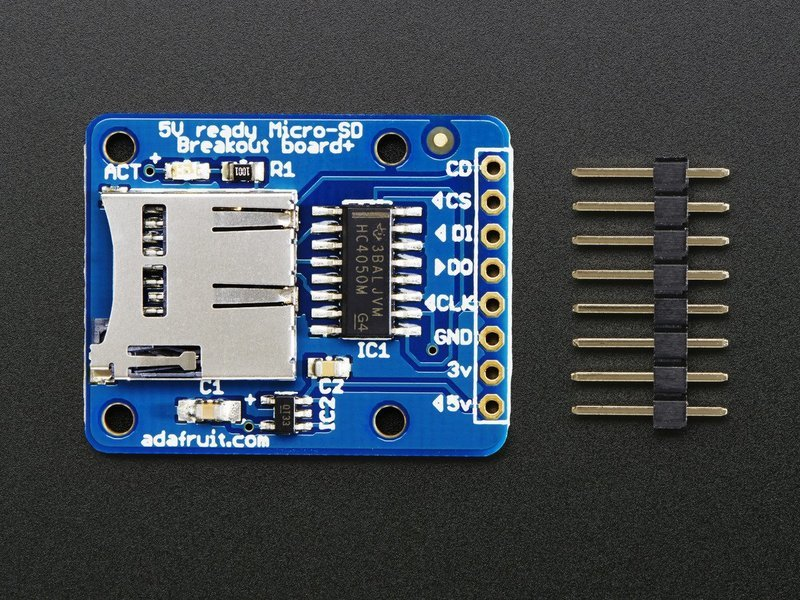
\includegraphics[width=0.5\linewidth]{graphics/Datenspeicherung/micro_sd_card_breakout.png}
\caption{254 $\mu$SD-Breakoutboard von Adafruit \cite{ladyada2018}}
\label{fig:muSDBreakout}
\end{figure}

\subsubsection{Verdrahtung}
SD-Karten erfordern viel Datenübertragung. Deshalb kann die beste Leistung erbracht werden, wenn sie an die Hardware-SPI-Pins eines Mikrocontrollers angeschlossen werden. Dabei wird es wie folgt miteinander verbunden: \cite{ladyada2018}
\todo[inline]{Hier vielleicht noch das Schema hinzufügen wie es Hardwaremässig implementiert wird.}
\begin{itemize}
\item \textbf{5V} und \textbf{GND} Pins jeweils auf die \textbf{5V} und \textbf{GND} Pins des Arduino Mega Boards
\item \textbf{CLK} auf die Pinnummer \textbf{52}
\item \textbf{DO} auf die Pinnummer \textbf{50}
\item \textbf{DI} auf die Pinnummer \textbf{51}
\item \textbf{CS} auf die Pinnummer \textbf{53}
\end{itemize}
\newpage

\subsubsection{SPI (Serial Peripheral Interface)}
\label{subsubsec:spi}
\begin{minipage}{0.48\textwidth}
Das \textit{Serial Peripheral Interface} ist ein synchrones serielles Datenprotokoll (Datenbus) bestehend aus drei Datenleitungen zur Datenübertragung. Diese sind, wie in Abbildung \ref{fig:spi} zu sehen, \textbf{MISO} (Master In Slave Out), \textbf{MOSI} (Master Out Slave In) und \textbf{SCLK} (Serial Clock). Auf dem Breakoutboard (Abb. \ref{fig:muSDBreakout}) sind die Pins mit \textbf{DI} (Data In), \textbf{DO} (Data Out) und \textbf{CLK} (Clock) beschrieben. Zu den Datenleitungen wird noch eine \textbf{SS}- (Slave Select) oder auch \textbf{CS}-Leitung (Chip Select) benötigt. Damit wird vom Master aus den zur momentanen Kommunikation nötigen Slave selektiert. Große Vorteile von SPI sind die Vollduplexfähigkeit und das Taktfrequenzen bis in den MHz-Bereich reichen. \cite{spi}\cite{Wikipedia2018spi}\\
\end{minipage}
\begin{minipage}{0.51\textwidth}
\centering
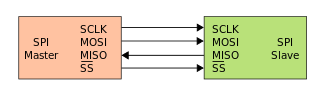
\includegraphics[width=\textwidth]{graphics/Datenspeicherung/spi_master_slave.png}
\captionof{figure}{Einfacher SPI-Datenbus \cite{Wikipedia2018spi}}
\label{fig:spi}
\end{minipage}
\todo[inline]{Möglicherweise noch die Taktfrequenz angeben, resp. die Einstellungen des SPI-Protokolls}

\subsection{$\mu$SD-Karte}
\begin{minipage}{0.44\textwidth}
\centering
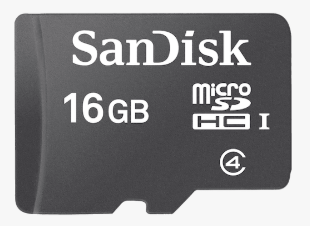
\includegraphics[width=0.4\textwidth]{graphics/Datenspeicherung/micro_sd_card_16GB.png}
\captionof{figure}{16 GB $\mu$SD-Karte \cite{musdkarte}}
\label{fig:muSDKarte}
\end{minipage}
\begin{minipage}{0.55\textwidth}
Bei der $\mu$SD-Karte muss auf die Kompatibilität mit dem Breakoutboard geachtet werden. Dafür sind folgende Kriterien zu beachten:\\
\begin{itemize}
\item Die $\mu$SD-Karte muss FAT16 oder FAT 32 formatiert sein.
\item Es sind nur die SD und SD High Capacity (SDHC) kompatibel.\\
\end{itemize}
\end{minipage}
Für die Umsetzung dieses Projektes wurde eine $\mu$SD-Karte der SD-Familie SDHC \Romannum{1} verwendet (siehe Abb. \ref{fig:muSDKarte}). SDHC sind Kapazitäten bis zu 32GB möglich und FAT32 formatiert. \cite{muSDspez} \todo[inline]{Es könnte noch auf die Anschlüsse der $\mu$SD-Karte eingegangen werden. Gäbe aber nur Sinn wenn ein Print erstellt werden muss wo das Breakoutboar nachkonstruiert wird.}
\newpage

\subsection{Implementation in die Firmware}
Für die Implementation in die Firmware, um mit dem Breakoutboard über SPI zu kommunizieren und die $\mu$SD-Karte zu beschreiben, resp. zu lesen, wurden direkt die bereits existierenden Librarys <SPI.h>\footnote{ <*.h> bezieht sich auf ein include-Verzeichnis unter dem Compiler-Installationsverzeichnis} und <SD.h> von Arduino inkludiert. In der Arduino IDE können bereits vorgefertigte Expample-Codes (siehe Abb. \ref{fig:exampleCodes}) zur weiteren Interpretation, wie mit diesen Librarys $\mu$SD-Karten gelesen und geschrieben werden können, verwendet werden.\\
\begin{figure}[h]
\centering
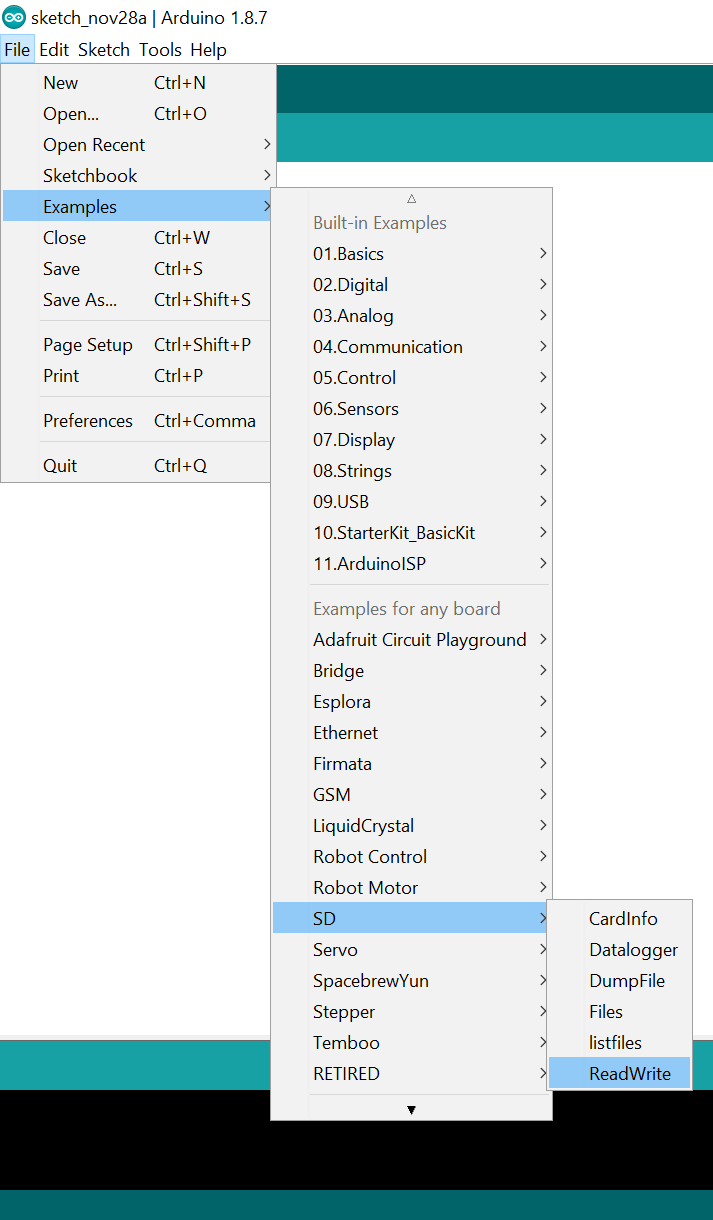
\includegraphics[width=0.5\textwidth]{graphics/Datenspeicherung/read_write_examples.PNG}
\caption{Example-Codes der Arduino IDE zum Lesen und Schreiben von SD-Karten.}
\label{fig:exampleCodes}
\end{figure}

Für eine übersichtlichere Programmstruktur und einfachere Handhabung wurden die Exampel-Codes für die korrekte Implementation angepasst und in Funktionen verpackt. Die Funktionen sind extern im Headerfile ''SDCard.h''\footnote{ ''*.h'' bezieht sich relativ auf das aktive Projektverzeichnis} deklariert und im SDCard.cpp initialisiert.\todo{Funktionen könnten noch beschrieben werden.}
\begin{itemize}
\item \textcolor{blue}{void} \textcolor{orange}{getCardInformations}():
\item \textcolor{blue}{void} \textcolor{orange}{readFileSDCard}(\textcolor{Dandelion}{String} filename): 
\item \textcolor{blue}{void} \textcolor{orange}{writeFileSDCard}(\textcolor{blue}{double} value2save, \textcolor{Dandelion}{String} filename): 
\item \textcolor{blue}{void} \textcolor{orange}{deleteFileSDCard}(\textcolor{Dandelion}{String} filename): 
\end{itemize}
\section{Kommunikationsmodul}

\section{Energieversorgung}

\section{Konzeptvalidierung}


%%---BIBLIOGRAPHY------------------------------------------------------------------------
\bibliography{literature/bibliography}

%%---APPENDIX----------------------------------------------------------------------------
\begin{appendix}
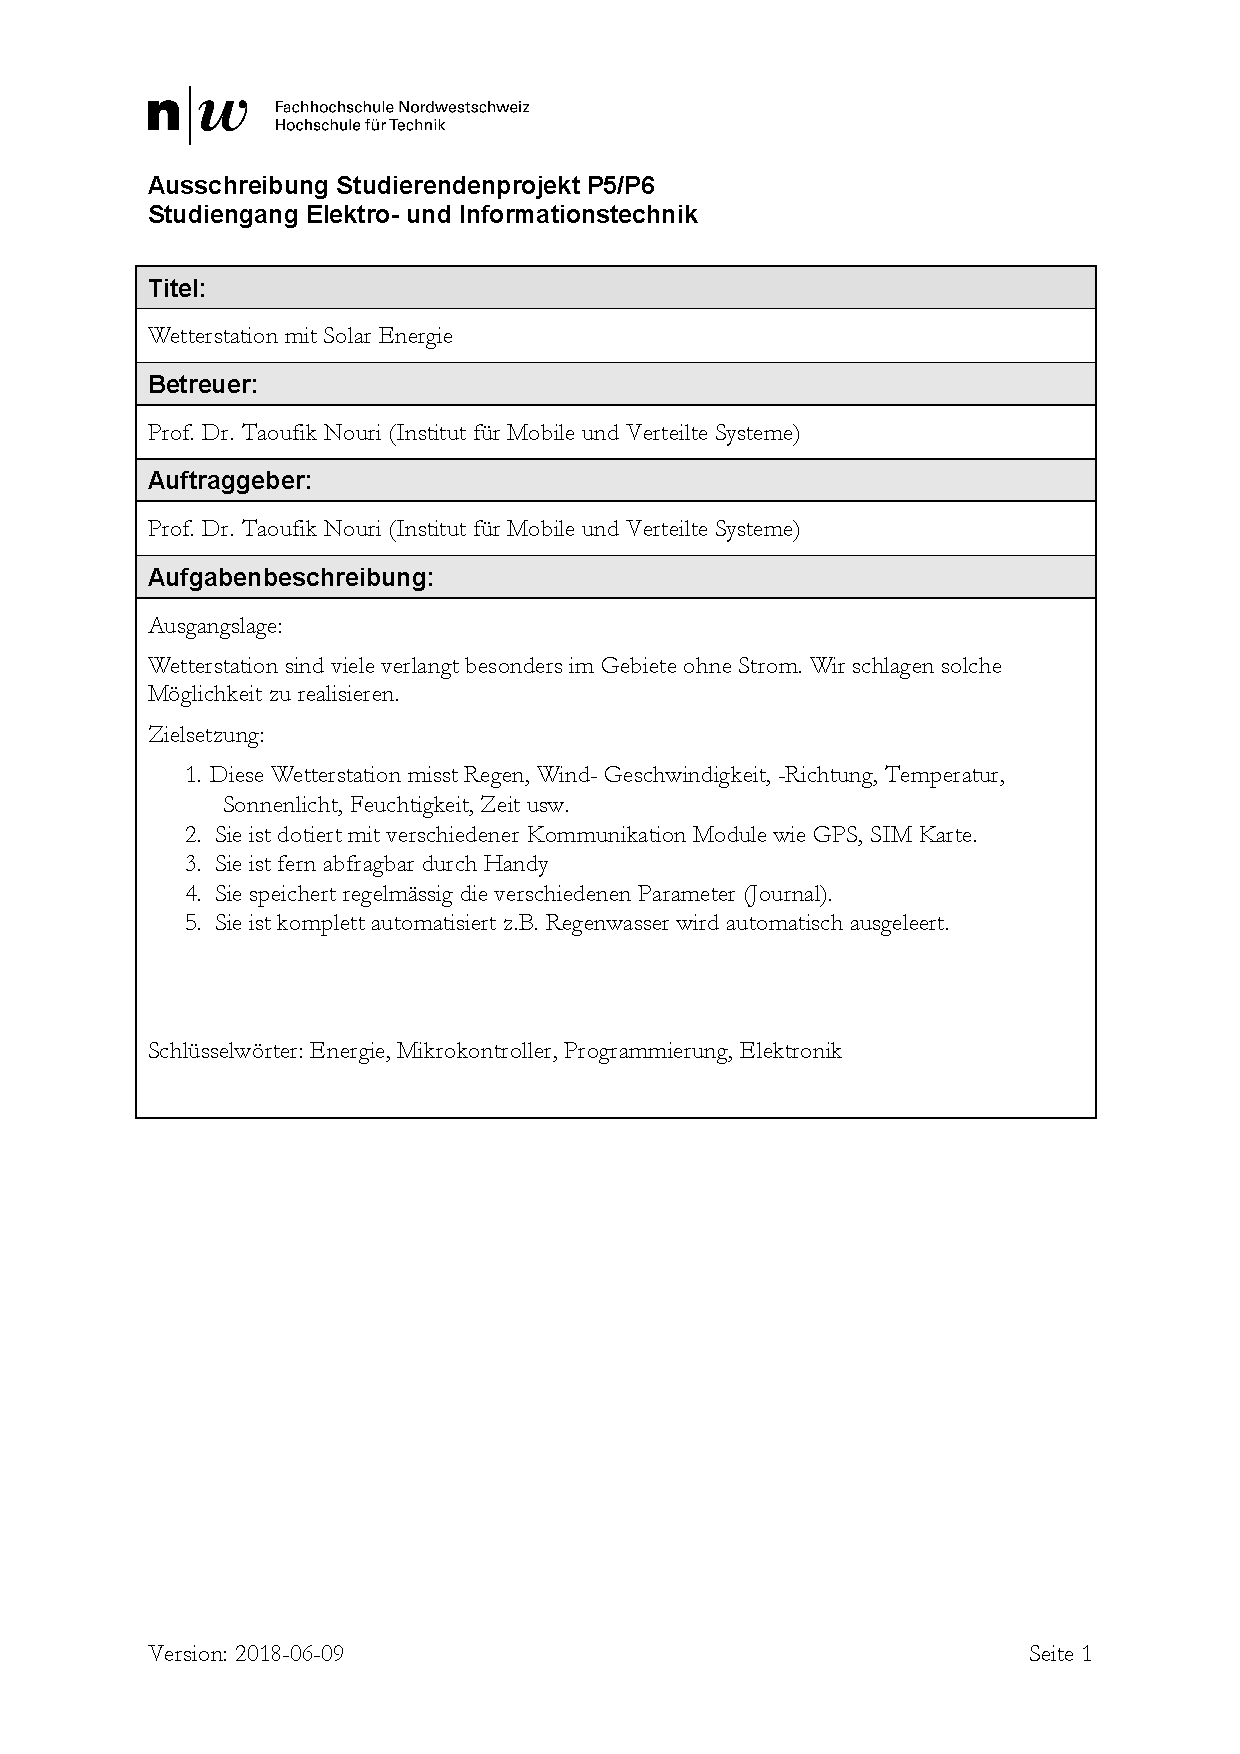
\includepdf[pages={1},nup=1x1,landscape=false,scale=0.85,offset=0 -40,pagecommand={\section{Lastenheft}\label{tab:zeitplan}\thispagestyle{myheadings}}]{appendix/Auftragsbeschreibung.pdf} 
\newpage

\section{ATmega2560-Arduino Pin Mapping}
\label{sec:pinMapping}
\begin{table}[h]
  \centering
  \caption{ATmega2560-Arduino Pin Mapping Tabelle \cite{ArduinoPinMapping2018}}
    \begin{tabular}{|c|p{15.855em}|p{11.43em}|}
    \hline
    \multicolumn{1}{|p{7.07em}|}{\textbf{Pin Number}} & \textbf{Pin Name} & \textbf{Mapped Pin Name} \\
    \hline
    1     & PG5 ( OC0B ) & Digital pin 4 (PWM) \\
    \hline
    2     & PE0 ( RXD0/PCINT8 ) & Digital pin 0 (RX0) \\
    \hline
    3     & PE1 ( TXD0 ) & Digital pin 1 (TX0) \\
    \hline
    4     & PE2 ( XCK0/AIN0 ) & \multicolumn{1}{l|}{} \\
    \hline
    5     & PE3 ( OC3A/AIN1 ) & Digital pin 5 (PWM) \\
    \hline
    6     & PE4 ( OC3B/INT4 ) & Digital pin 2 (PWM) \\
    \hline
    7     & PE5 ( OC3C/INT5 ) & Digital pin 3 (PWM) \\
    \hline
    8     & PE6 ( T3/INT6 ) & \multicolumn{1}{l|}{} \\
    \hline
    9     & PE7 ( CLKO/ICP3/INT7 ) & \multicolumn{1}{l|}{} \\
    \hline
    10    & VCC   & VCC \\
    \hline
    11    & GND   & GND \\
    \hline
    12    & PH0 ( RXD2 ) & Digital pin 17 (RX2) \\
    \hline
    13    & PH1 ( TXD2 ) & Digital pin 16 (TX2) \\
    \hline
    14    & PH2 ( XCK2 ) & \multicolumn{1}{l|}{} \\
    \hline
    15    & PH3 ( OC4A ) & Digital pin 6 (PWM) \\
    \hline
    16    & PH4 ( OC4B ) & Digital pin 7 (PWM) \\
    \hline
    17    & PH5 ( OC4C ) & Digital pin 8 (PWM) \\
    \hline
    18    & PH6 ( OC2B ) & Digital pin 9 (PWM) \\
    \hline
    19    & PB0 ( SS/PCINT0 ) & Digital pin 53 (SS) \\
    \hline
    20    & PB1 ( SCK/PCINT1 ) & Digital pin 52 (SCK) \\
    \hline
    21    & PB2 ( MOSI/PCINT2 ) & Digital pin 51 (MOSI) \\
    \hline
    22    & PB3 ( MISO/PCINT3 ) & Digital pin 50 (MISO) \\
    \hline
    23    & PB4 ( OC2A/PCINT4 ) & Digital pin 10 (PWM) \\
    \hline
    24    & PB5 ( OC1A/PCINT5 ) & Digital pin 11 (PWM) \\
    \hline
    25    & PB6 ( OC1B/PCINT6 ) & Digital pin 12 (PWM) \\
    \hline
    26    & PB7 ( OC0A/OC1C/PCINT7 ) & Digital pin 13 (PWM) \\
    \hline
    27    & PH7 ( T4 ) & \multicolumn{1}{l|}{} \\
    \hline
    28    & PG3 ( TOSC2 ) & \multicolumn{1}{l|}{} \\
    \hline
    29    & PG4 ( TOSC1 ) & \multicolumn{1}{l|}{} \\
    \hline
    30    & RESET & RESET \\
    \hline
    31    & VCC   & VCC \\
    \hline
    32    & GND   & GND \\
    \hline
    33    & XTAL2 & XTAL2 \\
    \hline
    34    & XTAL1 & XTAL1 \\
    \hline
    35    & PL0 ( ICP4 ) & Digital pin 49 \\
    \hline
    \end{tabular}%
  \label{tab:ATmega2560-Arduino Pin Mapping Tabelle}%
\end{table}%
\newpage
% Table generated by Excel2LaTeX from sheet 'Tabelle1'
\begin{table}[h]
  \centering
    \begin{tabular}{|c|p{15.855em}|p{11.43em}|}
    \hline
    \multicolumn{1}{|p{7.07em}|}{\textbf{Pin Number}} & \textbf{Pin Name} & \textbf{Mapped Pin Name} \\
    \hline
    36    & PL1 ( ICP5 ) & Digital pin 48 \\
    \hline
    37    & PL2 ( T5 ) & Digital pin 47 \\
    \hline
    38    & PL3 ( OC5A ) & Digital pin 46 (PWM) \\
    \hline
    39    & PL4 ( OC5B ) & Digital pin 45 (PWM) \\
    \hline
    40    & PL5 ( OC5C ) & Digital pin 44 (PWM) \\
    \hline
    41    & PL6   & Digital pin 43 \\
    \hline
    42    & PL7   & Digital pin 42 \\
    \hline
    43    & PD0 ( SCL/INT0 ) & Digital pin 21 (SCL) \\
    \hline
    44    & PD1 ( SDA/INT1 ) & Digital pin 20 (SDA) \\
    \hline
    45    & PD2 ( RXDI/INT2 ) & Digital pin 19 (RX1) \\
    \hline
    46    & PD3 ( TXD1/INT3 ) & Digital pin 18 (TX1) \\
    \hline
    47    & PD4 ( ICP1 ) & \multicolumn{1}{l|}{} \\
    \hline
    48    & PD5 ( XCK1 ) & \multicolumn{1}{l|}{} \\
    \hline
    49    & PD6 ( T1 ) & \multicolumn{1}{l|}{} \\
    \hline
    50    & PD7 ( T0 ) & Digital pin 38 \\
    \hline
    51    & PG0 ( WR ) & Digital pin 41 \\
    \hline
    52    & PG1 ( RD ) & Digital pin 40 \\
    \hline
    53    & PC0 ( A8 ) & Digital pin 37 \\
    \hline
    54    & PC1 ( A9 ) & Digital pin 36 \\
    \hline
    55    & PC2 ( A10 ) & Digital pin 35 \\
    \hline
    56    & PC3 ( A11 ) & Digital pin 34 \\
    \hline
    57    & PC4 ( A12 ) & Digital pin 33 \\
    \hline
    58    & PC5 ( A13 ) & Digital pin 32 \\
    \hline
    59    & PC6 ( A14 ) & Digital pin 31 \\
    \hline
    60    & PC7 ( A15 ) & Digital pin 30 \\
    \hline
    61    & VCC   & VCC \\
    \hline
    62    & GND   & GND \\
    \hline
    63    & PJ0 ( RXD3/PCINT9 ) & Digital pin 15 (RX3) \\
    \hline
    64    & PJ1 ( TXD3/PCINT10 ) & Digital pin 14 (TX3) \\
    \hline
    65    & PJ2 ( XCK3/PCINT11 ) & \multicolumn{1}{l|}{} \\
    \hline
    66    & PJ3 ( PCINT12 ) & \multicolumn{1}{l|}{} \\
    \hline
    67    & PJ4 ( PCINT13 ) & \multicolumn{1}{l|}{} \\
    \hline
    68    & PJ5 ( PCINT14 ) & \multicolumn{1}{l|}{} \\
    \hline    
    69    & PJ6 ( PCINT 15 ) & \multicolumn{1}{l|}{} \\
    \hline
    70    & PG2 ( ALE ) & Digital pin 39 \\
    \hline
    71    & PA7 ( AD7 ) & Digital pin 29 \\
    \hline
    72    & PA6 ( AD6 ) & Digital pin 28 \\
    \hline
    73    & PA5 ( AD5 ) & Digital pin 27 \\
    \hline
    74    & PA4 ( AD4 ) & Digital pin 26 \\
    \hline
    75    & PA3 ( AD3 ) & Digital pin 25 \\
    \hline
    76    & PA2 ( AD2 ) & Digital pin 24 \\
    \hline
    77    & PA1 ( AD1 ) & Digital pin 23 \\
    \hline
    78    & PA0 ( AD0 ) & Digital pin 22 \\
    \hline
    79    & PJ7   & \multicolumn{1}{l|}{} \\
    \hline
    80    & VCC   & VCC \\
    \hline
    \end{tabular}%
\end{table}%
% Table generated by Excel2LaTeX from sheet 'Tabelle1'
\begin{table}[h]
  \centering
    \begin{tabular}{|c|p{15.855em}|p{11.43em}|}
    \hline
    \multicolumn{1}{|p{7.07em}|}{\textbf{Pin Number}} & \textbf{Pin Name} & \textbf{Mapped Pin Name} \\
    \hline
    81    & GND   & GND \\
    \hline
    82    & PK7 ( ADC15/PCINT23 ) & Analog pin 15 \\
    \hline
    83    & PK6 ( ADC14/PCINT22 ) & Analog pin 14 \\
    \hline
    84    & PK5 ( ADC13/PCINT21 ) & Analog pin 13 \\
    \hline
    85    & PK4 ( ADC12/PCINT20 ) & Analog pin 12 \\
    \hline
    86    & PK3 ( ADC11/PCINT19 ) & Analog pin 11 \\
    \hline
    87    & PK2 ( ADC10/PCINT18 ) & Analog pin 10 \\
    \hline
    88    & PK1 ( ADC9/PCINT17 ) & Analog pin 9 \\
    \hline
    89    & PK0 ( ADC8/PCINT16 ) & Analog pin 8 \\
    \hline
    90    & PF7 ( ADC7 ) & Analog pin 7 \\
    \hline
    91    & PF6 ( ADC6 ) & Analog pin 6 \\
    \hline
    92    & PF5 ( ADC5/TMS ) & Analog pin 5 \\
    \hline
    93    & PF4 ( ADC4/TMK ) & Analog pin 4 \\
    \hline
    94    & PF3 ( ADC3 ) & Analog pin 3 \\
    \hline
    95    & PF2 ( ADC2 ) & Analog pin 2 \\
    \hline
    96    & PF1 ( ADC1 ) & Analog pin 1 \\
    \hline
    97    & PF0 ( ADC0 ) & Analog pin 0 \\
    \hline
    98    & AREF  & Analog Reference \\
    \hline
    99    & GND   & GND \\
    \hline
    100   & AVCC  & VCC \\
    \hline
    \end{tabular}%
\end{table}%

\begin{figure}[h]
\centering
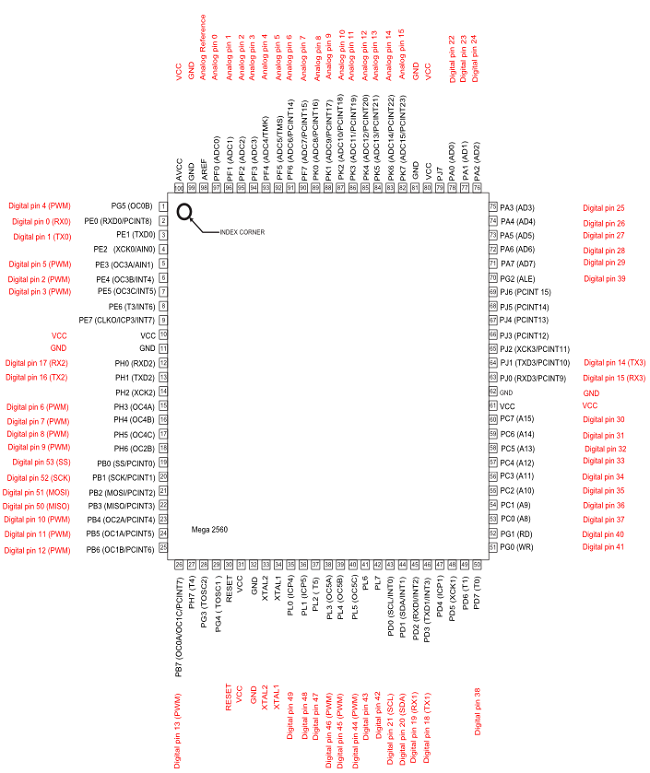
\includegraphics[width=\textwidth]{graphics/MCU/atmega2560_pins.png}
\caption{ATmega2560 Pin Layout}
\label{fig:ATmega2560PinLayout}
\end{figure}


\end{appendix}

%%---NOTES for DEBUG---------------------------------------------------------------------
\ifdraft{%Do this only if mode=draft
%%requires \usepackage{todonotes})
\newpage
\listoftodos[\section{Todo-Notes}]
\clearpage
}
{%Do this only if mode=final
}
\end{document}
